
\documentclass{beamer}


\mode<presentation>
{
  \usetheme{CambridgeUS}
	\usecolortheme{beaver}
  % or ...

  \setbeamercovered{transparent}
  % or whatever (possibly just delete it)
}


\usepackage{xeCJK}
\usepackage[english]{babel}
\usepackage[utf8]{inputenc}
\usepackage{times}
\usepackage[T1]{fontenc}
\usepackage{hyperref}
\usepackage{pifont}
\usepackage{bibentry}
\usepackage{verbatim}
\usepackage{color}
\newcommand{\cmark}{\ding{51}}%
\newcommand{\xmark}{\ding{55}}%
\setCJKmainfont{WenQuanYi Micro Hei}
\renewcommand{\raggedright}{\leftskip=0pt \rightskip=0pt plus 0cm}
\raggedright

\let\oldfootnotesize\footnotesize
\renewcommand*{\footnotesize}{\oldfootnotesize\tiny}


\title[开源软件基础] 
{开源软件基础}
\subtitle{Python动态分析}

\author[Zhilei Ren] 
{Zhilei Ren}

\institute[OSCAR Team] % (optional, but mostly needed)
{
\\
\includegraphics[width=0.2\textwidth]{../../utils/logo.jpg}\\
OSCAR Team, School of Software, 
Dalian University of Technology
}


\subject{Open source}



\pgfdeclareimage[height=0.5cm]{university-logo}{../../utils/logo.jpg}
\logo{\pgfuseimage{university-logo}}



% Delete this, if you do not want the table of contents to pop up at
% the beginning of each subsection:
\AtBeginSubsection[]
{
  \begin{frame}<beamer>{Outline}
    \tableofcontents[currentsection,currentsubsection]
  \end{frame}
}


% If you wish to uncover everything in a step-wise fashion, uncomment
% the following command: 

%\beamerdefaultoverlayspecification{<+->}

\setbeamertemplate{section in toc}[circle]
\setbeamertemplate{items}[circle]
\setbeamertemplate{caption}[numbered]
\setbeamertemplate{bibliography item}{\insertbiblabel}
\setbeamertemplate{bibliography entry title}{}
\setbeamertemplate{bibliography entry journal}{}

\begin{document}

\begin{frame}
  \titlepage
\end{frame}

%\begin{frame}{Outline}
%  \tableofcontents[currentsection,currentsubsection, 
%    hideothersubsections, 
%    sectionstyle=show,
%]
%\end{frame}

\AtBeginSection[]
{
 \begin{frame}<beamer>
 \frametitle{Outline}
 \tableofcontents[currentsection]
 \end{frame}
}

\section{inspect}

\begin{frame}[t]{Python的作用域}

    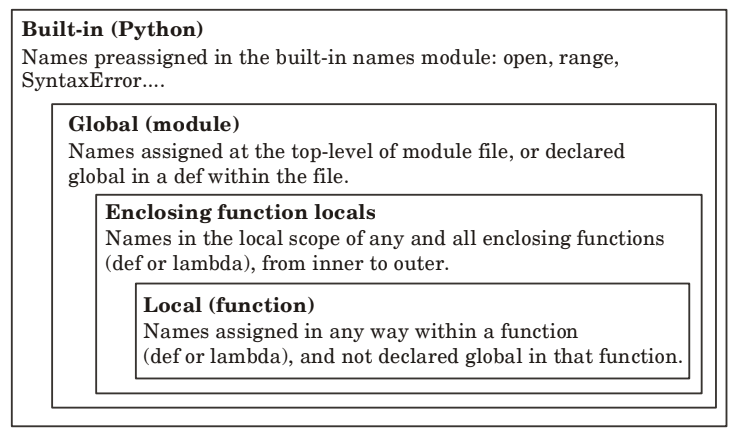
\includegraphics[width=0.6\textwidth]{legb.png}

	
\end{frame}

\begin{frame}[t,fragile]{inspect}
\begin{verbatim}
>>> import inspect
>>> def foo():
...     x = 10
...     return inspect.currentframe()
>>> f = foo()
>>> dir(foo)
['__class__',
  ... 
 'f_back',
 'f_builtins',
 'f_code',
 'f_globals',
 'f_lineno',
 'f_locals',
 'f_trace']
\end{verbatim}

	
\end{frame}

\begin{frame}[t]{inspect}

    \begin{table}
        \caption{frame成员}
    \begin{tabular}{ll}
        \hline
        成员 & 描述 \\
        \hline
f\_back & next outer frame object (this frame's caller) \\

f\_builtins & builtins namespace seen by this frame \\

f\_code & code object being executed in this frame \\

f\_globals & global namespace seen by this frame \\

f\_lasti & index of last attempted instruction in bytecode \\

f\_lineno & current line number in Python source code \\

f\_locals & local namespace seen by this frame \\

f\_trace & tracing function for this frame, or None	\\
        \hline
\end{tabular}
\end{table}
\end{frame}

\begin{frame}[t,fragile]{inspect}
\begin{verbatim}

x = 10
def outer():
    x = 20
    def inner():
        x = 30
        print(x)
        return inspect.currentframe()
    return inner
inn = outer()
frame = inn()
print(frame.f_locals['x'])
print(frame.f_globals['x'])
print(inspect.getclosurevars(inn))

\end{verbatim}

	
\end{frame}
\begin{frame}[t,fragile]{inspect}
\begin{verbatim}

x = 10
def outer():
    x = 20
    def inner():
        # x = 30
        print(x)
        return inspect.currentframe()
    return inner
inn = outer()
frame = inn()
print(frame.f_locals['x'])
print(frame.f_globals['x'])
print(inspect.getclosurevars(inn))

\end{verbatim}

	
\end{frame}
\section{sys.settrace}


\begin{frame}[t,fragile]{settrace}
\footnotesize
\begin{verbatim}
from sys import settrace
  
def tracer(frame, event, arg = None):
    code = frame.f_code
    func_name = code.co_name
    line_no = frame.f_lineno
    print(f"事件：{event}，函数：{func_name}()，行号：{line_no}")
    return tracer

def foo():
    print("in foo")

def bar():
    foo()

old_tracer = settrace(tracer)
bar()
settrace(old_tracer)
\end{verbatim}
\end{frame}
\end{document}
